\section{Abstract Syntax Tree}
\label{sec:AST}
As described in section \ref{sec:compiler}, the parser generates an abstract syntax tree (AST). An AST is a representation of the syntax in a programming language in the structure of a tree. Each node of the tree representates a token in the given sentence or code block. Since the tree is abstract not every single syntactic construct is shown in the tree. As javaCC is used in the creation of this project, the AST is generated automatically based on the grammar of the source language.

\subsection{AST for Function and Variable Declaration}
\begin{lstlisting}[caption=Function with variable declaration, label=lst:ast_func]
	void function Procedure() do
		int h = 10 + 11;
		string hello = "World!";
	end
\end{lstlisting}
\begin{figure}[H]
	\centering
		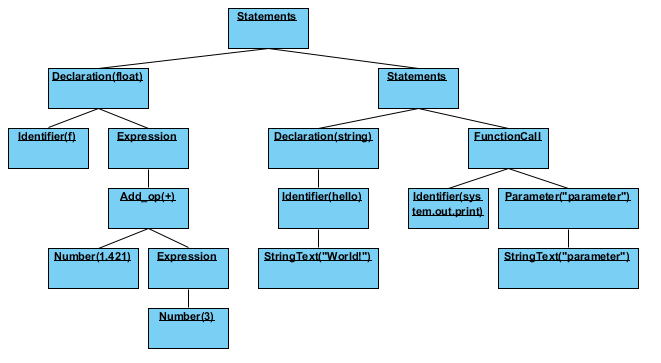
\includegraphics[width=\textwidth]{billeder/function_AST.png}
		\caption{AST for listing \ref{lst:ast_func}}
		\label{fig:ast_func}
\end{figure}
In listing \ref{ast_func} is seen a function with two different variable declarations in the source language. Figure \ref{fig:ast_func} shows the AST generated by javaCC using the beforementioned code example. It is not concrete to the specific token. As seen in the AST there are different opportunities for declaring a variable in the source language.

\subsection{AST for While Loops and If Statements}
\begin{lstlisting}[caption=While loop with if-statement, label=lst:ast_while]
	while(b <= i) do
		if(a EQUALS s) do
			string ok = "works!";
		end
	end
\end{lstlisting}
\begin{figure}[H]
	\centering
		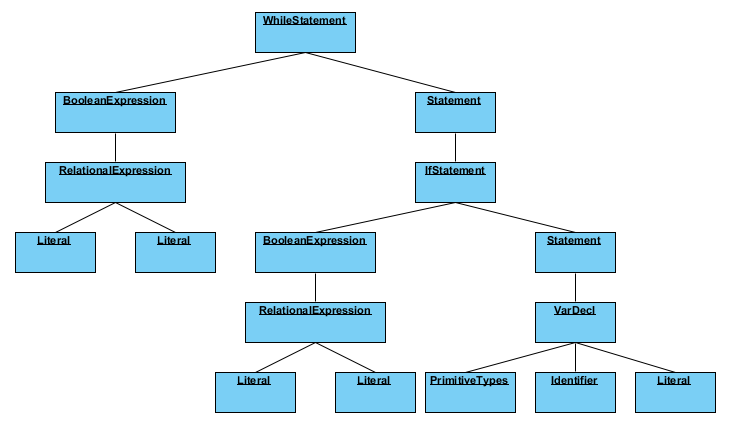
\includegraphics[width=\textwidth]{billeder/while_AST.png}
		\caption{AST for listing \ref{lst:ast_while}}
		\label{fig:ast_while}
\end{figure}
In listing \ref{lst:ast_while} is seen a while loop with an if-statement in the source language. Figure \ref{fig:ast_while} shows the AST generated from the code example.